\documentclass[12pt]{article}
\usepackage{anyfontsize}
\usepackage[a4paper, margin=2cm]{geometry}
\usepackage{polski}
\usepackage{tabto}
\usepackage{enumitem}
\usepackage{amsmath}
\usepackage{amssymb}
\usepackage{multirow}
\usepackage{multicol}
\usepackage{setspace}
\input{verticalPages.tex}


\usepackage{tabularx}
\newcolumntype{C}{>{\centering\arraybackslash}X}
\newcolumntype{L}{>{\raggedleft\arraybackslash}X}
\newcolumntype{R}{>{\raggedright\arraybackslash}X}
\newcommand{\centerY}[2]{\multirow{#1}{*}{#2}}

\usepackage{wrapfig}

\usepackage{chngcntr}
\counterwithin{figure}{section}
\counterwithin{table}{section}
\numberwithin{equation}{section}

\usepackage{hyperref}
\hypersetup{
    colorlinks = true,
    urlcolor=blue,
    linkcolor= black
}

\usepackage{graphicx}
\graphicspath{{./Img/}}

\usepackage{csvsimple}
\usepackage{pgfplots}
\usepackage{pgfplotstable}
\pgfplotsset{compat= newest}


\usepackage{titlesec}
\titlelabel{\thetitle.\quad}
% \AddToHook{cmd/section/before}{\clearpage}

\usepackage[european, american currents, americanvoltages, RPvoltages, cute inductor]{circuitikz}
\usepackage{tikz}
\usetikzlibrary{shapes.geometric}
\ctikzset{
    logic ports=ieee,
    logic ports/scale=0.7,
}

\title{
    \includegraphics[width = 0.3\textwidth]{agh_logo.jpg}\\
    \textbf{Akademia górniczo-hutnicza w Krakowie}\\
    Wydział Informatyki, Elektroniki i  Telekomunikacji\\\vspace{2cm}
    \textbf{Praca inżynierska}\\
    Pojazd autonomiczny z możliwością oceny aktualnej sytuacji na drodze\\\vspace{1cm}
    \small{Autonomous vehicle with ability to assess current road situation}
}
\author{
    \begin{tabularx}{\textwidth}{l l}
    Autorzy: &Łukasz Przystupa\\
    Kierunek studiów: & Elektronika\\
    Opiekun pracy: &dr inż. Agnieszka Dąbrowska-Boruch
    \end{tabularx}
}
\date{\vspace{2cm}\today}

\usepackage{titling}
\renewcommand\maketitlehooka{\null\mbox{}\vfill}
\renewcommand\maketitlehookd{\vfill\null}

\begin{document}
    \begin{titlepage}
        \maketitle
        \thispagestyle{empty}
        \newpage
        \ 
        \thispagestyle{empty}
    \end{titlepage}
    
    \pagenumbering{Roman}
        \section*{Spis skrótów}
\addcontentsline{toc}{section}{Spis skrótów}
\begin{table*}[!ht]
    \begin{tabularx}{\textwidth}{|c|C|C|}\hline
        Skrót & Rozszerzenie\ & Opis\\\hline
        \centerY{2}{GPIO}       & \centerY{2}{General Purpose Input/Output} & Wyprowadzenia z układów scalonych do dowolnego wykorzystania\\\hline
        \centerY{2}{DIY}        & \centerY{2}{Do It Yourself} & Projekt do własnoręcznego wykonania\\\hline
        \centerY{2}{SSH}        & \centerY{2}{Secure Shell} & Protokół komunikacyjny, pozwalający na bezpieczne połączenie do serwera\\\hline
        \centerY{2}{HAL}        & \centerY{2}{Hardware Abstraction Layer} & Sposób porozumiewania się ze sprzętem\\\hline
        \centerY{3}{PWM}        & \centerY{3}{Pulse Wave Modulation} & Rodzaj modulacji cyfrowych pozwalający na regulację wypełnienia sygnału\\\hline
        \centerY{3}{ToF}        & \centerY{3}{Time of Flight} & Rodzaj czujników pomiaru odległości, polegający na pomiarze czasu przelotu wiązki światła\\\hline
        \centerY{1}{IR}         & \centerY{1}{Infrared} & Czujniki wykrywające promieniowanie podczerwone\\\hline
        \centerY{2}{CAD}        & \centerY{2}{Computer Aided Design} & Zestaw narzędzi do projektowania np.~modeli 3D\\\hline
        \centerY{1}{RB Pi Pico} & \centerY{1}{Raspberry Pi Pico} & Mikrokontroler firmy Raspberry Pi\\\hline
    \end{tabularx}
\end{table*}
        \tableofcontents
        \newpage
    \pagenumbering{arabic}
    % \input{Chapters/Abstract.tex}
    \section{Wstęp}
    Celem poniższej pracy jest skonstruowanie autonomicznego pojazdu, którego zadaniem będzie zbudowanie wirtualnej mapy terenu oraz samodzielne poruszanie się po nieznanym obszarze.
    Jednym z założeń projektu jest umożliwienie użytkownikowi kontroli nad pojazdem za pomocą dedykowanej aplikacji komputerowej.
    Dodatkowo, powyższa aplikacja będzie wyświetlać budowaną mapę w czasie rzeczywistym.
    Po wskazaniu punktu docelowego, zostanie zaproponowana optymalna trasa, po której pojazd będzie się poruszał.


    \subsection{Środowisko sprzętowe}
        Współczesne pojazdy autonomiczne wyposażone są w jednostki obliczeniowe, które swoją konstrukcją przypominają pełnoprawne komputery z systemem operacyjnym.
        Ten projekt ma być modelem,  przedstawiającym działanie pojazdu autonomicznego, dlatego wykorzystanie pełnoprawnego komputera jest zbędne.

        \subsubsection{Mikrokontroler}
            Poniżej przedstawiono kilka najbardziej popularnym platform sprzętowych, które mogą stanowić bazę dla pojazdu.
            \begin{enumerate}
                \item Raspberry Pi -- komputer z systemem operacyjnym Linux, umożliwiający bezpośredni dostęp do modułów zewnętrznych z pomocą GPIO.
                Jest to najbardziej popularna platforma dla projektów DIY.
                Układ pozwala na niesamowitą elastyczność w pracy, między innymi na podłączenie się do układu za pośrednictwem SSH oraz pracę w języku Python.
                Jednak ze względu na swoją popularność, jest bardzo drogi i mało dostępny.
                Natomiast, jednym z założeń projektu jest działanie w czasie rzeczywistym, co przy wykorzystaniu systemu operacyjnego jest niemożliwe.
                \item Arduino -- najpopularniejsza platforma, której głównymi zaletami są: prostota framework'u oraz mnogość bibliotek dla każdego układu.
                Niestety, płytki te oparte są o 8-bitowe mikrokontrolery z rodziny AVR, co odbija się na ich prędkościach  (max 20MHz).
                Sam framework wykorzystywany jest na wielu różnych praformach, przez co w dłuższej perspektywie staje się nieintuicyjny.
                \item STM32 -- układy projektowane przez firmę STMicroelectronics. Są znacznie szybsze i posiadają więcej pamięci od Arduino.
                Jednak ze względu na potrzebę wykorzystania biblioteki HAL, programowanie jest znacznie trudniejsze w porównaniu do innych układów.
                \item ESP32 -- 32-bitowy dwurdzeniowy procesor z wbudowanym modułem WiFi i Bluetooth.
                Jeden z najszybszych mikrokontrolerów dostępnych na rynku. Jest bardzo popularny w projektach IoT (wytłumaczyć).
                Natywnie pracuje w systemie czasu rzeczywistego - FreeRTOS. Dzięki temu ma potencjał na bycie idealnym kandydatem do tego projektu.
                Jednak znikoma dokumentacja produktu sprawia, że praca z nim jest uciążliwa, przez co opracowanie optymalnego kodu jest znacząco utrudnione.
                \item Raspberry Pi Pico -- mikrokontroler od firmy Raspberry Pi, oparty na rdzeniach Cortex - tak samo jak STM32.
                Producent udostępnił wyjątkowo przystępny zestaw narzędzi programistycznych oraz przykładów użycia.
                Kolejną z zalet jest dobra dokumentacja tego procesora, która jest stale rozwijana.
                W 2022 roku, pojawiła się druga iteracja tej płytki Raspberry Pi Pico~W ze zintegrowanym modułem WiFi.
            \end{enumerate}
            Projekt jest możliwy do zrealizowania na wszystkich wymienionych powyżej platformach.
            Jednak ze względu na swoją przystępność, Raspberry Pi Pico jest najbardziej optymalnym wyborem.
            \begin{figure}[!ht]
                \centering
                \includegraphics[width = 0.3\textwidth]{raspberry_pico.png}
                \caption{Raspberry Pi Pico}
                Źródło: \href{https://botland.com.pl/moduly-i-zestawy-do-raspberry-pi-pico/21574-raspberry-pi-pico-w-rp2040-arm-cortex-m0-cyw43439-wifi-5056561803173.html}{botland.com}

                % Źródło: https://botland.com.pl/silniki-dc-z-przekladnia-i-enkoderami/6287-silnik-z-przekladnia-sj01-120-1-6v-160rpm-enkoder-6959420910205.html
                % Źródło: https://botland.com.pl/serwa-typu-micro/20435-serwo-mg-90s-micro-180-stopni-metalowa-przekladnia-5904422380915.html
                \label{fig:raspberry_pico}
            \end{figure}

        \subsubsection{Sterowanie}
        \label{sec:engines}
            Podstawowym zadaniem pojazdów mechanicznych jest poruszanie się.
            Dlatego niezwykle istotne było wybranie odpowiedniego silnika napędowego.
            Na rynku konsumenckim istnieje jest wiele ich wariantów.
            Poniżej opisano możliwe rozwiązania oraz skrótowo omówiono ich wady i zalety:
            \begin{enumerate}
                \item Silniki krokowe -- niegdyś bardzo duże i drogie silniki, wymagające dodatkowych układów sterujących.
                Dziś jednak istnieją mniejsze, niskonapięciowe rozwiązania, które mogą być kontrolowaneZ bezpośrednio przez mikroprocesor.
                Niestety złożone sterowanie oraz niewielka prędkość maksymalna $v_{max} \approx 1 \frac{\text{obr.}}{s}$ sprawiają, że wykorzystanie ich w tym projekcie byłoby nieoptymalne.
                \item Serwomechanizmy $360^\circ$ -- silniki wraz z kontrolerem oraz przekładniami.
                Wbudowany układ pozwala na regulację prędkości z wysoką dokładnością.
                Nie ma jednak możliwości sprawdzenia, czy dwa moduły pracują z tą samą mocą.
                Może to prowadzić do wielu niepożądanych zachowań, jak na przykład trudności poruszaniem się w linii prostej.
                \item Serwomechanizmy $180^\circ$ -- ta odmiana pozwala na precyzyjne ustawienie pożądanego kąta.
                Układy te nie nadają się do napędzania pojazdów, gdyż ich zakres ruchu jest ograniczony do 180(stopni). Jednak, świetnie odnajdują się w sytuacjach, w których precyzja jest kluczowa.
                \item Silniki BLDC -- pozwalają osiągnąć bardzo wysokie prędkości.
                Niestety łączy się to z niemałą ceną.
                Dodatkowo każdy silnik wymaga wyspecjalizowanych układu sterującego.
                \item Silniki DC -- urządzenia elektromechaniczne przetwarzające moc prądu stałego na energię mechaniczną.
                Pozwalają na regulację prędkości za pomocą PWM.
                Dodatkowo w sprzedaży dostępne są układy wyposazone w enkodery, pozwalające obliczyć średnią prędkość silnika, a w konsekwencji wyznaczyć różnicę w pracy między nimi.
            \end{enumerate}
            Układ napędowy został oparty na silnikach DC z zamontowanymi enkoderami.
            Dzięki czemu możliwy jest odczyt prędkości pojazdu, który pozwala na wprowadzanie korekty szybkości.
            Natomiast, do układu kierowniczego, najlepiej nada się serwomechanizm $180^\circ$, ze względu na możliwość precyzyjnego ustawienia kąta. Oba wybrane układy przedstawiono poniżej \ref{fig:engines}.
            \begin{figure}[!ht]
                \centering
                \includegraphics[width = 0.3\textwidth]{silnik_z_enkoder.png}
                \includegraphics[width = 0.3\textwidth]{serwo_180.png}

                \caption{Silnik DC z enkoderem oraz serwomechanizmy $180^\circ$.}
                \footnotesize{Źródło: \href{https://botland.com.pl/}{botland.com}}
                % Źródło: https://botland.com.pl/silniki-dc-z-przekladnia-i-enkoderami/6287-silnik-z-przekladnia-sj01-120-1-6v-160rpm-enkoder-6959420910205.html
                % Źródło: https://botland.com.pl/serwa-typu-micro/20435-serwo-mg-90s-micro-180-stopni-metalowa-przekladnia-5904422380915.html
                \label{fig:engines}
            \end{figure}

        \subsubsection{Pomiar odległości}
            Praca pojazdów autonomicznych nie ogranicza się wyłącznie do sterowania silnikami.
            Urządzenia tego typu muszą być świadome swojego otoczenia.
            Zastosowanie odpowiednich czujników umożliwiających pomiar odległości jest niezbędne w celu zapewnienia bezkolizyjnej jazdy.
            % Autonomia pojazdu nie ogranicza się wyłącznie do sterowania silnikami.
            % Pojazd tego typu musi być świadomy swojego otoczenia.
            % Taką funkcjonalność mogą zapewnić czujniki służące do pomiaru odległości.
            % Ta funkcja wymaga wykorzystania czujników pozwalających na pomiar odległości.
            Poniżej przedstawiono listę różnych rodzajów czujników:
            \begin{enumerate}
                \item Czujniki ultradźwiękowe -- najpopularniejsze układy wykorzystywane do pomiaru odległości.
                Niewątpliwą zaletą jest prostota działania, jednak okupiona jest ona długim czasem wykonywania pomiarów.
                Co więcej uzyskane wartości obarczone są niepewnością, skutkującą znacznym odchyleniem od średniej.
                % Co więcej ich pomiary bywają niestabilne.
                \item Czujniki Time of Flight (ToF) -- wyspecjalizowane moduły o wysokiej dokładności, pozwalają na pomiary na znacznych odległościach.
                Zazwyczaj wymagają odpowiednich bibliotek dostarczonych przez producentów, co stanowi zarówno wadę jak i zaletę.
                Takie czujniki mogą pracować bardzo szybkie jednak złożona, uniwersalna biblioteka spowalnia cały proces.
                \item Układy obiciowe IR -- obwody składające się z dwóch diod, emitera i odbiornika.
                Cechują się niewielkim zakresem pomiarowym (od $2cm$ do $20cm$) i znikomą dokładnością (pomiar zależy od koloru obiektu) oraz zauważalną strefą martwą.
                \item Lidar -- wyspecjalizowane układy, umożliwiające bardzo precyzyjny określenie odległości w pełnym zakresie $360^\circ$.
                Sprawia to że jest jedną z najlepszych dostępnych opcji, jednak ceny takich układów są zaporowe.
                \item Radar -- niezwykle dokładne i kosztowne układy pomiarowe, pozwalające na nieporównywalną precyzję.
                Niestety ich rozmiar wymagany do tego projektu jest trudno dostępny na rynku konsumenckim.
                Co gorsza obowiązkowym staje się zastosowanie specjalnych procesorów sygnałowych, pozwalających na bieżąco przetwarzać dane z radarów.
            \end{enumerate}
            % Z wyżej przedstawionej listy, układami które sprawdzą się najlepiej w tym projekcie są czujniki typu ToF, zamontowane z przodu pojazdu.
            Z wyżej przedstawionej listy, w tym projekcie najlepiej sprawdzą się moduły ToF, zamontowane z przodu pojazdu.
            Dodatkowo ze względów bezpieczeństwa, z tyłu umieszczone zostały czujniki IR.
            Natomiast, nie są one wykorzystywane w charakterze urządzenia pomiarowego, tylko jako czujniki zbliżeniowe, umożliwiające wykrycie przeszkody i reakcję na niebezpieczeństwo.

    \subsection{Środowisko programistyczne}
        Następnym kluczowym wyborem jest środowisko programistyczne, w którym zostanie zbudowany projekt.
        % W ostatnich latach użytkownicy dostali bardzo dużo wolności w tej kwestii.
        W ostatnich latach powstało wiele narzędzi, pozwalających na dostosowanie całości do własnych potrzeb.
        Najpopularniejszymi narzędziami do programowania mikrokontrolerów są:
        \begin{enumerate}
            \item Eclipse -- kiedyś bardzo popularny program, posiadający olbrzymi zbiór dodatków.
            Rozprowadzany na otwartej licencji, dlatego stanowi doskonałą bazę dla wielu bardziej zaawansowanych projektów.
            \item STM32 Cube -- środowisko przeznaczone głównie do pracy z modułami STM32, oparte na wyżej wymienionym Eclipse.
            \item Microchip Studio -- zbiór narzędzi wyspecjalizowanych do pracy z mikrokontrolerami z rodziny AVR od firmy Microchip.
            \item Keil µVision -- program do programowania procesorów Cortex. Pomimo ograniczonej licencji jest bardzo popularny.
            \item Notepad++ -- bardziej zaawansowany notatnik, pozwalający na autouzupełnianie słów.
            Posiada też masę wtyczek, umożliwiających stworzenie z niego pełnoprawnego środowiska programistycznego, jednak w swojej pierwotnej wersji bardzo toporny w użyciu.
            \item VS Code -- uniwersalne narzędzie, mające ogrom dodatków, które dają możliwość przystosowania edytor w pełni pod własne wymagania.
            Sam program zbudowany jest na silniku przeglądarki internetowej, dzięki czemu może z powodzeniem zastąpić jej funkcje takie jak: przeglądarka PDF, a wbudowany tile menedżer pozwala układać całość w bardzo czytelny sposób.
        \end{enumerate}
        Projekt został, zbudowany z wykorzystaniem programu VS Code, ze względu na największą elastyczność oraz możliwość dostosowania go do własnych potrzeb.


    \subsection{Środowisko CAD}
        Zbudowanie pojazdu autonomicznego wymaga wymodelowania odpowiednich części.
        % Dodatkowo, praca wymagała zaprojektowania kilku dodatkowych elementów mechanicznych.
        W tym celu, zostało wykorzystane środowisko CAD, które pozwala na zaprojektowanie modelu 3D.
        Poniżej przedstawiono trzy najpopularniejsze programów do projektowania.
        \begin{enumerate}
            \item SolidWorks -- program stworzony przez firmę Dassault Systemes, który jest bardzo popularny w przemyśle. Jest też niezwykle precyzyjny i każda operacja wymaga zastanowienia się dokładnie co chce się osiągnąć - przez co próg wejścia jest bardzo wysoki.
            \item Fusion 360 -- program stworzony przez firmę Autodesk, przeznaczony specjalnie do modelowania 3D. Posiada olbrzymie wsparcie dla drukarek 3D, a także dla obrabiarek CNC.
                                Jest także niezwykle intuicyjny a próg wejścia jest bardzo niski. Jedyną wadą programu, jest możliwość jedynie pracy w chmurze.
            \item FreeCAD -- darmowy program do projektowania modeli 3D, bardzo prosty w obsłudze, a nauczenie się tego programu wymaga naprawdę niewielkiego wkładu pracy.
                             Program jest stale rozwijany, a społeczność wokół niego ma możliwość rozbudowywania go o nowe funkcje. Niewątpliwą zaletą w porównaniu do innych programów jest możliwość uruchomienia go na każdym systemie operacyjnym.
        \end{enumerate}

        W projekcie został wykorzystany program FreeCAD, ze względu na swoją prostotę oraz możliwość uruchomienia na systemie Linux.


        \useNormalLandscape
\lsection{Schemat blokowy}
    Na schemacie blokowym \ref{schema:block}, przedstawiono przepływ sygnałów sterujących, wraz z poszczególnymi blokami.
\begin{figure}[!ht]
\centering
\vspace{1cm}
\begin{circuitikz}[fill = white]
    \draw[very thick]
        (0, 0) node[draw, rectangle, fill, minimum width = 4cm, minimum height = 4cm, align = center] (MCU) {Mikrokontroler\\\scriptsize{Raspberry PI PICO W}}

        (0, -5) node[draw, rectangle, fill, minimum width = 3cm, minimum height = 3cm, align = center] (HBridge){Mostek H}
        (HBridge.south) ++(1, 0) --++(0, -1) to[Telmech=M, n = LMotor] ++ (2, 0) --++ (0, 2) --++ (-2, 0)
        (HBridge.south) ++(-1, 0) --++(0, -1) to[Telmech=M,n = RMotor] ++ (-2, 0) --++ (0, 2) --++ (2, 0)

        (-10, 4) node[draw, rectangle, fill, minimum width = 2cm, minimum height = 2cm, align = center] (ToF1) {$\text{ToF}_1$}
        (-7, 4) node[draw, rectangle, fill, minimum width = 2cm, minimum height = 2cm, align = center] (ToF2) {$\text{ToF}_2$}
        (-4, 4) node[draw, rectangle, fill, minimum width = 2cm, minimum height = 2cm, align = center] (ToF3) {$\text{ToF}_3$}

        (-6, 0) node[draw, rectangle, fill, minimum width = 2cm, minimum height = 2cm, align = center] (MPU6050){MPU6050\\lub\\MPU6000}
        (-6, -4) node[draw, rectangle, fill, minimum width = 2cm, minimum height = 2cm, align = center] (Magneto){Magnetometr}

        (6, -4) node[draw, rectangle, fill, minimum width = 2cm, minimum height = 2cm, align = center] (LIR){Czujnik\\cofania}
        (9, -4) node[draw, rectangle, fill, minimum width = 2cm, minimum height = 2cm, align = center] (RIR){Czujnik\\cofania}

        (6, 4) node[elmech=M, scale = 1.5](servo){S}
        (8, 0) node[draw, rectangle, fill, minimum width = 2cm, minimum height = 2cm, align = center] (memory) {Pamięć}
    ;

    \draw[]
        (MCU.east) to[bmultiwire = 4, a = SPI] (memory.west)
        (MCU.east) ++ (0, 1) to[short, i=PWM] ++ (4, 0) -| (servo.south)
        (MCU.east) ++ (0,-1) to[bmultiwire = 2] ++ (2, 0) --++ (0, -1) to[short, i<= Detect, -*]++ (2, 0) coordinate(IR_node)
            (IR_node)  to[multiwire=1] (LIR.north)
            (IR_node)  to[multiwire=1] ++ (3, 0)-| (RIR.north)
    
        (MCU.south) to[tmultiwire=6, i=\ ] (HBridge.north)

        (MCU.west) to[bmultiwire = 2, a = I2C, -*] ++ (-2, 0) coordinate(I2C) 
        (I2C) -- (MPU6050.east)
        (I2C) |- (Magneto)

        (I2C) to[short, -*] ++ (0, 2) coordinate(I2C)
        (I2C) -- (ToF3.south)
        (I2C) to[short, -*]++ (-3, 0) coordinate(I2C) -- (ToF2.south)
        (I2C) -| (ToF1)

        (LMotor) to[crossing] ++ (0, 4) --++ (0, 0.5) to[bmultiwire, a = 2] ++ (-1, 0) --++ (0, 1)
        (RMotor) to[crossing] ++ (0, 4) --++ (0, 0.5) to[bmultiwire = 2] ++ ( 1, 0) --++ (0, 1)
    ;
\end{circuitikz}
\renewcommand{\figurename}{Schemat}
\caption{Schemat blokowy, przedstawiający przepływ sygnałów w projekcie}
\label{schema:block}
\end{figure}
    \useportrait
% \footnote{Pamięć dodatkowa do przechowywania map terenu}

    \section{Budowa pojazdu}
\label{sec:building}
    Inspiracją do stworzenia poniższego projektu były samochody autonomiczne, które najczęściej są pojazdami dwuosiowymi, z jedną osią skrętną i jedną napędową.
    Żadna z nich nie jest ze sobą połączona, co pozwoliło na niezależne sterowanie.
    W konstrukcji zostały użyte dwa silniki prądu stałego, wybrane w rozdziale \ref{sec:engines}, połączone bezpośrednio do tylnych kół.
    \subsection{Przednia oś}
    \label{subsec:drive_axis}
        Układ kierowniczy oparto na serwomechanizmie.
        Na rysunku \ref{fig:frontAxis_model} przedstawiono model tego elementu, zaprojektowanego przez autora.

        \begin{figure}[!ht]
            \centering
            \includegraphics[width=0.7\textwidth]{FronAxis_example.png}
            \caption{Przykładowy układ kierowniczy zaprojektowany w narzędziu FreeCAD}
            \label{fig:frontAxis_model}
        \end{figure}
        Mechanizm ten został rozplanowany w taki sposób, aby środek osi znajdował się w linii ze środkiem serwomechanizmu.
        Dzięki temu ustawiony kąt serwa, odpowiada kątowi skrętu kół.
        Natomiast dużą wadą takiego połączenia jest możliwość jego uszkodzenia, po przekroczeniu maksymalnego zakresu ruchu.

    \subsection{Rama pojazdu}
    Do budowy podwozia została wykorzystana gotowa rama, z poniższego zdjęcia (rys. \ref{fig:test_chassis}), produkowana przez firmę Waveshare.
\clearpage
    \begin{figure}[!ht]
        \centering
        \includegraphics[width=0.7\textwidth]{chassis-waveshare-24419.png}
        \caption{Rama Waveshare 24419}
        Źródło: \href{https://www.waveshare.com/robot-chassis.htm?sku=24419}{waveshare.com}
        \label{fig:test_chassis}
    \end{figure}

    Aby spełnić założenia projektowe, przednia oś konstrukcji została wymieniona na wyżej opisaną (rozdział \ref{subsec:drive_axis}).
    Dodatkowo zmieniono sposób montażu silników, które zamontowano odwrotnie do zaleceń producenta (rys. \ref{fig:motors}), a także zrezygnowano z ,,gumek", odpowiadających za amortyzację.

    \begin{figure}[!ht]
    \centering
    \begin{subfigure}{0.49\textwidth}
        \centering
        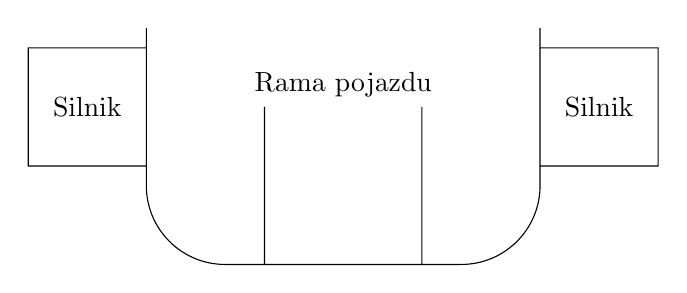
\begin{tikzpicture}
            \draw
                (0, 0) -- ++ (0, -2)
                    arc(0:90:-1)
                    -- ++ (3, 0)
                    arc(-90:0:1)
                    -- ++ (0, 2)

                (0, -0.25) rectangle node[]{Silnik} ++(-1.5, -1.5)
                (5, -0.25) rectangle node[]{Silnik} ++( 1.5, -1.5)


                (1.5, -3) --++(0, 2)
                (3.5, -3) --++(0, 2)
                (2.5, -1) node[above]{Rama pojazdu}
            ;
        \end{tikzpicture}
        \caption{Pierwotne połączenie}
    \end{subfigure}
    \begin{subfigure}{0.49\textwidth}
        \centering
        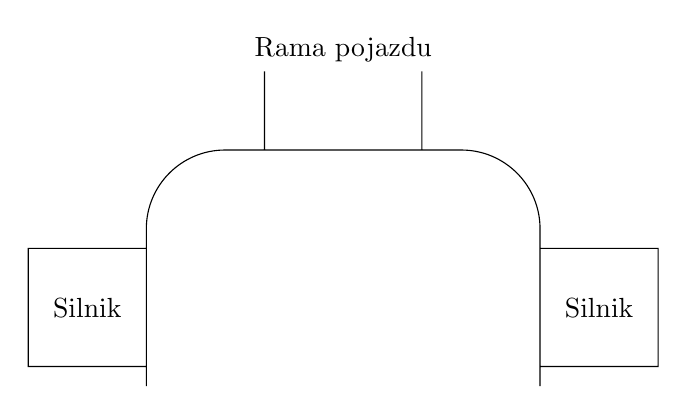
\begin{tikzpicture}
            \draw
                (0, 0) -- ++ (0, 2)
                    arc(0:-90:-1)
                    -- ++ (3, 0)
                    arc(90:0:1)
                    -- ++ (0,-2)

                (0, 0.25) rectangle node[]{Silnik} ++(-1.5, 1.5)
                (5, 0.25) rectangle node[]{Silnik} ++( 1.5, 1.5)

                (1.5, 3) --++(0, 1)
                (3.5, 3) --++(0, 1)
                (2.5, 4) node[above]{Rama pojazdu}
            ;
        \end{tikzpicture}
        \caption{Zastosowane połączenie}
    \end{subfigure}
    \caption{Schemat montażu silników}
    \label{fig:motors}
\end{figure}


    \subsection{Pomiar odległości}
        Współczesne pojazdy autonomiczne wykorzystują układy LIDAR, które pozwalają mierzyć w~pełnym zakresie $360^\circ$.
        Jednak w wielu sytuacjach taki pomiar mija się z celem, gdyż znaczna część próbek zostaje odrzucona.
        Same LIDARy zaś są bardzo drogimi urządzeniami, często z~niestandardowym sposobem komunikacji (np. za pomocą UART).
        Z tego względu autor zdecydował się na zastosowanie tańszych czujników ToF.
        Trzy takie moduły umieszczono z przodu samochodu, z krokiem co $30^\circ$.
        Na rysunku \ref{fig:ToF_holder} zaprezentowano model mocowania wyżej wymienionych elementów.

        \begin{figure}[!ht]
            \centering
            \includegraphics[width=0.7\textwidth]{ToF_holder.png}
            \caption{Mocowanie czujników ToF}
            \label{fig:ToF_holder}
        \end{figure}

    \section{Problemy konstrukcyjne}
\label{sec:problemy_konstrukcyjne}
    W poniższym rozdziale zostaną przedstawione problemy konstrukcyjne,
    które pojawiły się podczas realizacji projektu.

    \subsection{Jazda prosto}
    \label{section:jazda_prosto}
        Najprostszą czynnością każdego pojazdu jest jazda prosto.
        Operacja ta może wydawać się łatwa jednak wcale taka nie jest.
        Przykładowo kiedy usiądziemy za kierownicą, prawdziwego samochodu kontroluje podświadomie wiele parametrów takich jak:
        \begin{itemize}
            \item nachylenie terenu,
            \item aktualną pozycję kół,
            \item linie poziome na drodze czy pobocze drogi.
        \end{itemize}
        Jako ludzie wiele tych parametrów kontroluje ,,na wyczucie'' jednak pojazdy autonomiczne, są poniekąd robotami, które nie mogą polegać na ,,uczuciu'', że jadą prosto.
        Dlatego koniecznym jest zastosowanie odpowiednich czujników, które pozwolą na dokładną kontrolę jazdy.
        W poniższym rozdziale pokrótce zostaną opisane rozwiązanie dzięki którym samochód jest w stanie jeździć w sposób powtarzalny.

        \subsubsection{Różnica prędkości silników}
            Zastosowanie dwóch silników ma swoje wady i zalety.
            Niewątpliwą zaletą jest podwojenie mocy pojazdu.
            Jednak olbrzymią wadą okazało się sterowanie i nierównomierność pracy silników.
            Na wykresie \ref{plot:distance_err_in_time_const_speed} poniżej przedstawiono różnicę drogi pokonanej przez każdy silnik dla jednakowego sygnału sterującego.

            \begin{figure}[!ht]
                \centering
                \begin{tikzpicture}
                    \begin{axis}[
                        width = 0.7\textwidth,
                        grid = both,
                        grid style = dashed,
                        % axis lines = middle,
                        xlabel = czas ${[s]}$,
                        ylabel = różnica odległości ${[mm]}$,
                        xmin = 0,
                        xmax = 20,
                    ]
                        \addplot[blue] table[x = Time, y = Diff, col sep = comma]{Measure/distance_no_PID_speed_50.csv};
                        \legend{Błąd odległości}
                    \end{axis}
                \end{tikzpicture}
                \caption{Wykres różnicy przebytej drogi między prawym a lewym silnikiem bez regulacji}
                \label{plot:distance_err_in_time_const_speed}
            \end{figure}

            Aby rozwiązać powyższy problem należy zastosować regulator PID pozwalający w trakcie pracy, korygować prędkość silników.
            Natomiast podczas startu silników została zastosowana sztywna korekta prędkości w celu zminimalizowania błędu.
            \begin{figure}[!ht]
                \centering
                \begin{tikzpicture}
                    \begin{axis}[
                        width = 0.7\textwidth,
                        grid = both,
                        grid style = dashed,
                        xlabel = czas ${[s]}$,
                        ylabel = różnica odległości ${[mm]}$,
                        xmin = 0,
                        xmax = 60,
                    ]
                        \addplot[blue] table[x = Time, y = Distance_err, col sep = comma]{Measure/PID_speed_10.csv};
                        \legend{Błąd odległości}
                    \end{axis}
                \end{tikzpicture}
                \caption{Wykres różnicy przebytej drogi między prawym a lewym silnikiem z włączonym regulatorem PID. Prędkość pojazdu: $(35.10 \pm 0.10)\frac{mm}{s}$.}
                \label{plot:PID_distance_err_in_time}
            \end{figure}

            Jak widać na wykresie \ref{plot:PID_distance_err_in_time} w początkowej fazie, silniki nadal nie pracują równomiernie, w dłuższej perspektywie praca silników osypuje w okół stałej wartości $(0 \pm 3)mm$.

    \subsubsection{Nieidealność podwozia}
        Kolejnym napotkanym problemem, okazuje się nieidealność podwozia.
        Szczególnie elementu przedstawionego na rysunku \ref{fig:frontAxis_model} oraz nierównomierne rozłożenie masy względem środka.
        Wszystkie wyżej wymienione niedokładności powodowały, że pojazd cały czas skręcał w jedną stronę.
        Rozwiązaniem tego problemu jest zastosowanie pętli sprzężenia zwrotnego, opartej na czujniku $MPU6050$, który został użyty jak żyroskop, pozwalający na pomiar biedzącego kąta.
        Dzięki czemu można korygować kierunek skręcania pojazdu.

        Jednak jego wykorzystanie nie było bezproblemowe i wymagało dodatkowych poprawek.
        Na wykresie \ref{plot:gyro_magneto_measure} przedstawiono pomiar kąta dla obrotu pojazdu ze stałą prędkością w jednym kierunku po kalibracji czujnika.
        Poniższy pomiar został wykonany w celu ustalenia liniowości pracy żyroskopu opartego na akcelerometrze.
        Układem referencyjnym był uprzednio skalibrowany magnetometr (układ $QMC5883L$).
%
        \begin{figure}[!ht]
            \centering
                \begin{tikzpicture}
                    \begin{axis}[
                        width = 0.65\textwidth,
                        grid = both,
                        grid style = dashed,
                        xlabel = czas ${[s]}$,
                        ylabel = kąt zmierzony podczas obrotu ${[^\circ]}$,
                        ymin = -5,
                        ymax = 365,
                        xmin = 0,
                        xmax = 2.9,
                        ytick = {0, 30, ..., 360},
                        legend style={at={(0.2, 0.92)}, anchor=north},
                    ]
                        \addplot[orange] table[x = Time, y = Compass_azimuth, col sep = comma]{Measure/angles.csv};
                        \addplot[blue] table[x = Time, y = Gyro_z, col sep = comma]{Measure/angles.csv};
                        \legend{magnetometr,żyroskop}
                    \end{axis}
                \end{tikzpicture}
                \caption{Wykres pomiary azymutu za pomocą magnetometru oraz zmiany kąta wykazanego przez żyroskop}
                \label{plot:gyro_magneto_measure}
        \end{figure}
        Podczas pomiaru, na oba układy został nałożony filtr dolnoprzepustowy, eliminujący szumy.

        Wykres \ref{plot:delta_angle_with_gyro} przedstawia narastanie katą, mierzonego przez żyroskop.
        Widać bardzo dużą liniowość pracy żyroskopu, co pozwala zaufać temu czujnikowi na tyle, aby na jego podstawie określać czy pojazd jedzie prosto.

        % \begin{wrapfig}[!ht]
        \begin{figure}[!ht]
            \centering
                \begin{tikzpicture}
                    \begin{axis}[
                        width = 0.7\textwidth,
                        grid = both,
                        grid style = dashed,
                        xlabel = czas ${[s]}$,
                        ylabel = kąt zmierzony podczas obrotu ${[^\circ]}$,
                        xmin = 0,
                        xmax = 2.9,
                    ]
                        \addplot[blue] table[x = Time, y = Delta_angle, col sep = comma]{Measure/angles.csv};
                    \end{axis}
                \end{tikzpicture}
                \caption{Wykres narastania kąta, zmierzonego przez żyroskop}
                \label{plot:delta_angle_with_gyro}
        \end{figure}
        % \end{wrapfig}


% \newpage
    Oba wyżej opisane rozwiązania pozwalają na w miarę stałą jazdę prostą ($\pm 2^\circ$).
    A w sytuacjach, kiedy pojazd zaczyna znacząco skręcać na przykład po impakcie z boku, sprzężenie zwrotne z żyroskopu pozwala wykryć znaczącą zmianę kąta ruchu.
    Kolejny regulator PID odczytuje wartość kąta i koryguje kąt serwomechanizmu tak aby pojazd wrócił na prostą.

    \subsection{Skręcanie}
        Rozwiązanie problemów z jazdą prosto to tylko połowa sukcesu.
        Kolejne mankamenty wyszły podczas próby skręcania.
        Nie tylko w pierwotnej wersji nie było stałe - ustawienie stałego kąta kół oraz przejechanie tej samej drogi nie zawsze dawało ten sam rezultat.
        To pojazd cały czas miał tendencję do preferowania skrętu w jedną stronę.

        \subsubsection{Dyferencjał}
        \label{subsubsec:dyferencjal}
        Najprostszym do zauważenia problemem był brak dyferencjału.
        Tylna oś pojazdu posiada dwa silniki jednak w poprzednich testach, zostały one ,,software'owo połączona sztywną belką".
        Powodowało to poślizg pojazdu podczas skręcania a w konsekwencji uniemożliwiało powtarzalność manewru.

        Rozwiązaniem tego problemu jest zmiana prędkości pracy silników w zależności od promienia skrętu.
        Poniżej przedstawiono schemat algorytmu, na którego podstawie wyznaczono procentową wartość dyferencjału.
        Rysunek \ref{draw:turning_car} przedstawia schematyczną sytuację skręcania.
        \begin{figure}[!ht]
    \centering
    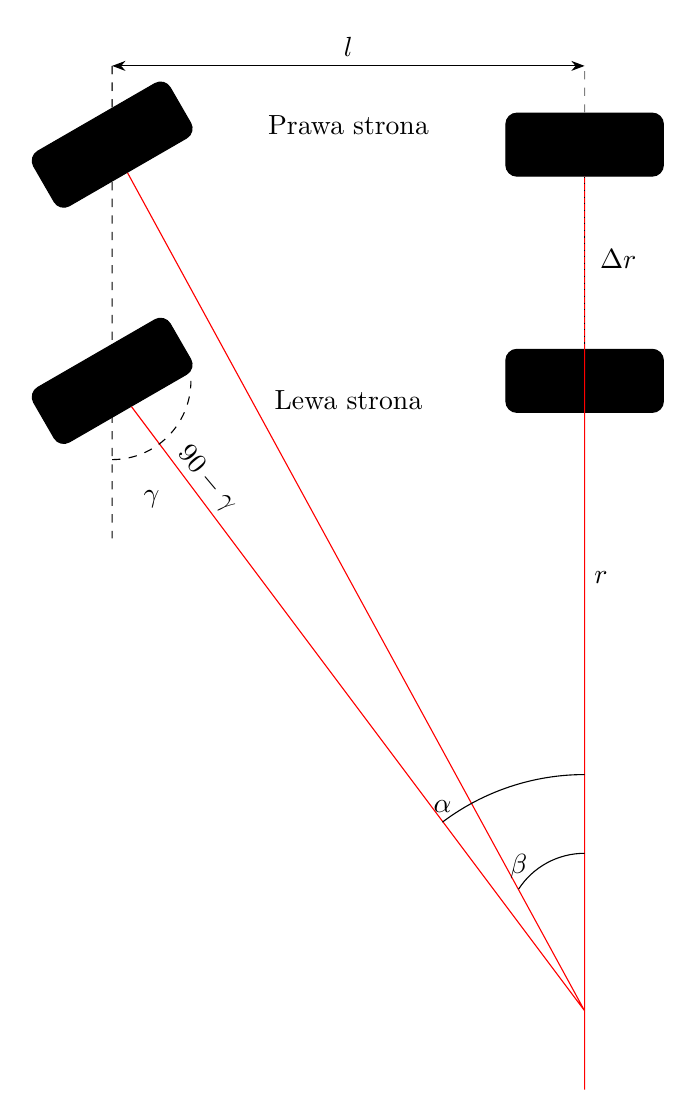
\begin{tikzpicture}
        \draw
            (0, 0) node[draw, rectangle, rounded corners, fill = black, minimum width = 2cm, minimum height = 0.8cm, rotate = 30](frontL){}
            (0, -3) node[draw, rectangle, rounded corners, fill = black, minimum width = 2cm, minimum height = 0.8cm, rotate = 30](frontR){} 
            
            (6, 0) node[draw, rectangle, rounded corners, fill = black, minimum width = 2cm, minimum height = 0.8cm](backL){}
            (6, -3) node[draw, rectangle, rounded corners, fill = black, minimum width = 2cm, minimum height = 0.8cm](backR){}

            (3, 0) node[above]{Prawa strona}
            (3,-3) node[below]{Lewa strona}
        ;

        \draw[Stealth-Stealth]
            (frontL) ++ (0, 1) --node[above]{$l$}++ (6, 0)
        ;
        \draw[dashed, gray]
            (frontL) --++(0, 1)
            (backL) --++(0, 1)
        ;

        \draw[color = red]
            (backL) -- ++ (0, -10) -- ++ (0, -1) coordinate(meet) --++ (0, -1)
            (frontL) -- (meet)
            (frontR) -- (meet)
        ;
        \draw
            (meet) ++ (0, 3) arc(90:127:3) node[above]{$\alpha$}
            (meet) ++ (0, 2) arc(90:147:1) node[above]{$\beta$}
        ;

        \draw[dotted]
            (backL) to[short, l=$\Delta r$] (backR)
            (backR) ++ (0, -2.5) node[right]{$r$}
        ;

        \draw[dashed]
            (frontL) ++ (0, 1) -- (0, -5)
            (0, -4) arc(90:180:-1)
            (0.5, -4.5) node[]{$\gamma$}
            (1.2, -4.25) node[rotate = -50]{$90 - \gamma$}
        ;
    \end{tikzpicture}
    \caption{Rysunek poglądowy do skręcenia}
    \label{fig:turning_car}
\end{figure}

        Jak widać skręt pojazdu można opisać jako ruch dwóch kół po okręgach o wspólnym środku, w których poszczególne prędkości liniowe nie są sobie równe.
        Jednak występuje zależność:
        \begin{gather}
            \omega_{\text{wewnęrznego koła}} = \omega_{\text{zewnętrznego koła}}\\
            \frac{v_{\text{wewnęrznego koła}}}{r} = \frac{v_{\text{zewnętrznego koła}}}{r + \Delta r}\\
            \frac{v_\text{wewnęrznego koła}}{v_{\text{zewnętrznego koła}}} = \frac{r}{r + \Delta r}
        \end{gather}

        Aby policzyć zależność między prędkościami silników, należy wyznaczyć promień skrętu.
        Do tego celu, można wykorzystać znane wartości i równanie \ref{eq:turning_radius}.
        Znanymi wartościami są:
        \begin{gather}
            \tan \left(90 - \gamma\right) = \frac{l}{r}\\
            r(\gamma) = \frac{l}{\tan(90-\gamma)}
            \label{eq:turning_radius}
        \end{gather}

        Gdzie:
        \begin{itemize}
            \item $l = 155$ -- długość między osiami samochodu:,
            \item $\Delta r = 125$ -- odległość między kołami w jednej osi,
            \item $\gamma \in <60^\circ \div 120^\circ>$ -- kąt skrętu kół, ustawiany przez algorytm nawigacji lub użytkownika.
        \end{itemize}

        A zatem procentowy stosunek prędkości w funkcji kąta można wyrazić jako:
        \begin{gather}
            \frac{v_{\text{prawe koła}}}{v_{\text{lewe koła}}} = 1 + \frac{\Delta r}{r} = 1 + \Delta r \cdot \frac{\tan(90 - \gamma)}{l}
        \end{gather}


        \subsection{Nierównomierność skrętu}
        \label{subsec:nierownomiernosc_skretu}
            W trakcie testów, okazało się że pojazd nie skręca równomiernie w obie strony.
%
            Podczas manewrów w prawo, na łuku o długości $s = 500mm$, pojazd zakreślał kąt około $70^\circ$.
            Natomiast na tym samym odcinku ale w lewo zakreślany kąt to około $50^\circ$.

            Wymusiło ustawienie wartości offsetu, przesuwającej wartość kąta skrętu.
            Jego wartość została wyznaczona eksperymentalnie i wynosiła około $-6^\circ$.
            Dla podanej wartości kąt zakreślany podczas skrecania w obu kierunkach wynosił około $60^\circ$.



    Dzięki wszystkim wyżej wymiennym zabiegom udało się uzyskać powtarzalne wyniki zarówno podczas jazdy prosto, cofania się oraz skręcania.
    Powyższe działania są niezbędne, jeśli budowany robot ma być sterowany autonomicznie.



    \vfill
    \begin{flushright}
        Łukasz Przystupa
    \end{flushright}
\end{document}
